\documentclass[10pt,conference,compsocconf]{IEEEtran}

\usepackage{hyperref}
\usepackage{graphicx}
\usepackage{booktabs}
\usepackage{amsmath}
\usepackage{xcolor}
\usepackage{tikz}
\usetikzlibrary{arrows.meta, positioning, fit, backgrounds, shapes.geometric, calc}

\begin{document}
\title{How Foveated Vision Shapes Cognitive Maps in Navigation Agents}

\author{
  Name1 (SCIPER1), Name2 (SCIPER2), Name3 (SCIPER3), Name4 (SCIPER4)\\
  \textit{CS-503 Visual Intelligence --- Project Proposal}
}

\maketitle

% ---------- Abstract ----------
\begin{abstract}
Cognitive maps emerge in the recurrent hidden states of navigation agents, as shown separately for blind agents with only GPS and compass and for agents with uniform visual input. Both are perceptual extremes. Real perception lies between them: biological vision is spatially non-uniform, and much of what the agent sees is imprecise by construction. A foveated sensor lets us ask a question that uniform vision hides: when an agent trained only to reach goals faces systematically unreliable peripheral observations, does its memory develop an internal representation of its \emph{own} observational uncertainty, even though the navigation loss contains no direct signal for uncertainty? If such uncertainty-tracking emerges, it does so because it is instrumentally useful for navigation under partial observability---a non-trivial claim about what navigation pressure alone can shape memory into. We test this by probing the hidden states of a foveated agent for per-location observation quality and by asking whether memory accuracy \emph{inverts} input quality (higher for peripherally-seen regions than foveated ones), with two ablations defending the comparison against confounds.
\end{abstract}


% ---------- Introduction ----------
\section{Introduction}

The cognitive map hypothesis~\cite{tolman1948cognitive}---that animals build internal spatial representations to support flexible navigation---is a long-standing idea in spatial cognition. Wijmans et al.~\cite{wijmans2023emergence} gave it a computational counterpart: reinforcement learning agents trained on PointGoal navigation develop map-like representations in their recurrent hidden states, detectable by linear probes that decode occupancy grids, agent position, and collision predictions. They showed that this occurs even in \emph{blind} agents receiving only GPS and compass---vision is not required for spatial memory to emerge.

This result characterises one end of the perceptual range. The other end---uniform high-resolution RGB---is what most embodied AI training assumes. Real biological vision is neither: humans see sharply only within the central $\sim$2\textdegree{} of gaze (the fovea), and resolution falls off rapidly with eccentricity. The agent must choose where to look, and the periphery feeds memory with information that is uncertain by construction. It is an open question whether a learned agent placed in this regime develops the same kind of cognitive map as a uniform-vision agent, or a different one that compensates for the uneven input.

\subsection{What is the problem?}

Existing probing studies of navigation agents~\cite{wijmans2023emergence,dwivedi2022isee} characterize \emph{what} cognitive maps emerge under uniform or absent vision; none vary the spatial quality of the visual input. As a result, we cannot tell whether the spatial concepts found in those hidden states are properties of the navigation task itself or artifacts of receiving every part of the scene at the same resolution. We ask: \textbf{when a navigation agent sees the world through a foveated sensor, what does it choose to remember, and does its memory reflect a strategy for managing perceptual uncertainty?}

\subsection{Why does this matter?}

\begin{itemize}
    \item \textbf{It asks whether navigation pressure alone can induce epistemic memory}\quad The navigation loss rewards reaching goals, not tracking how well one saw each region. A learned cognitive map could encode only the spatial layout, or it could, as a side effect of being useful for planning, also encode the agent's own observational uncertainty. Existing probing work~\cite{wijmans2023emergence,dwivedi2022isee} cannot tell these apart: under uniform vision, confidence is high everywhere and both accounts predict nearly identical probes. Foveation creates regions the agent could not see clearly, and the two accounts then diverge---a layout-only memory's accuracy should drop with eccentricity, while an uncertainty-annotated one should stay flat or \emph{rise}. Finding the latter would indicate that epistemic structure emerges in the hidden state without any explicit signal rewarding it.
    \item \textbf{It suggests a candidate answer to ``what should a memory store?''}\quad Recurrent policies for partial observability (LSTMs, Transformer memories) currently store whatever the loss pushes them toward, without a principled rule. If foveated agents develop uncertainty-driven storage (H1), that suggests a concrete inductive bias---weight memory updates by per-region observation quality---potentially portable to other memory modules for POMDP-style tasks.
    \item \textbf{It reframes learned gaze as a question about memory, not task performance}\quad Active-vision RL~\cite{lv2023sugarl} shows that learned gaze improves task return, but mostly treats gaze as a performance lever. Our H3 test asks whether the agent looks where its memory is weakest---a step toward a functional explanation of what the gaze policy is doing.
\end{itemize}


% ---------- Method ----------
\section{Method and Deliveries}

\subsection{Experimental design}

\textbf{Simulator and dataset}\quad We train all agents in Habitat~\cite{savva2019habitat}, a high-throughput 3D simulator that renders first-person RGB at thousands of frames per second, on the Gibson dataset~\cite{xia2018gibson} of photorealistic 3D reconstructions of real buildings. Specifically, we use the Gibson-0+ PointNav training split of Wijmans et al.~\cite{wijmans2020ddppo}, which contains 411 scenes with 10{,}000 pre-generated episodes per scene -- the largest publicly released Gibson PointNav episode set, and a 5.7$\times$ scene-diversity increase over the 72-scene Gibson-4+ default used by the public emergence-of-maps code release. The task is PointGoal navigation: the agent starts at a random pose and must reach a target specified as a displacement vector (distance and heading to goal) using discrete actions (\textsc{forward}, \textsc{turn-left}, \textsc{turn-right}, \textsc{stop}). For evaluation we follow Wijmans et al.~\cite{wijmans2023emergence}, Appendix A.1, and evaluate on the 18 Matterport3D test scenes with 56 episodes per scene (1008 episodes total), which serves as an out-of-dataset generalization test.

\textbf{Three agents, shared backbone}\quad All agents share an identical 3-layer LSTM (512-d) and the Wijmans sensor stack from Sec.\ A.1 of~\cite{wijmans2023emergence}: goal-in-start-frame, GPS, compass, and a close-to-goal indicator, each projected to 32-d and concatenated with a 32-d previous-action embedding before the LSTM. The conditions differ only in the visual input fed alongside this block, so any observed difference in memory content can be attributed primarily to sensor structure rather than to backbone or task:

\begin{figure}[tbph]
\centering
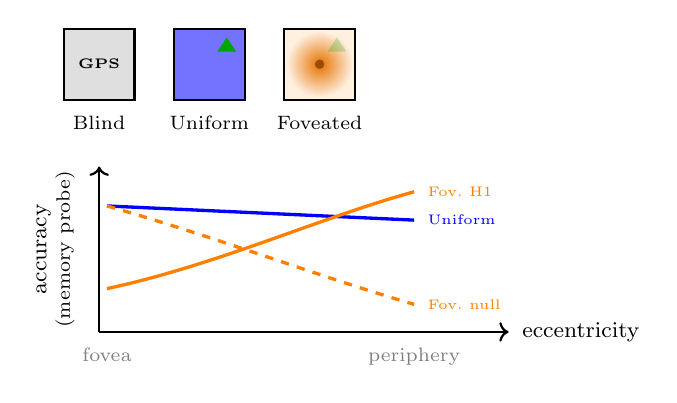
\begin{tikzpicture}[every node/.style={font=\scriptsize}]
% ============= TOP: three visual conditions (main) =============
% Each sighted panel renders the same scene object — a green triangle —
% at the same upper-right position. The conditions differ only in the
% *quality* of the rendering:
%   uniform  : full resolution, full clarity
%   foveated : full resolution, but blurred outside the central fovea

% Blind (gray) — no visual input, no object
\fill[gray!25] (-0.45,-0.45) rectangle (0.45,0.45);
\draw[thick] (-0.45,-0.45) rectangle (0.45,0.45);
\node at (0,0) {\tiny\textbf{GPS}};
\node at (0,-0.75) {Blind};

% --- Uniform (blue) — crisp triangle, full resolution ---
\fill[blue!55] (0.95,-0.45) rectangle (1.85,0.45);
\fill[green!65!black]
  (1.62,0.34) -- (1.50,0.16) -- (1.74,0.16) -- cycle;
\draw[thick] (0.95,-0.45) rectangle (1.85,0.45);
\node at (1.4,-0.75) {Uniform};

% --- Foveated (orange) — central fovea, periphery blurred, triangle faded ---
\begin{scope}
  \clip (2.35,-0.45) rectangle (3.25,0.45);
  \fill[orange!12] (2.35,-0.45) rectangle (3.25,0.45);
  \shade[inner color=orange!90!black, outer color=orange!12]
    (2.8,0) circle (0.42);
  \fill[orange!60!black] (2.8,0) circle (0.06);
  \fill[green!65!black, opacity=0.22]
    (3.02,0.34) -- (2.90,0.16) -- (3.14,0.16) -- cycle;
\end{scope}
\draw[thick] (2.35,-0.45) rectangle (3.25,0.45);
\node at (2.8,-0.75) {Foveated};

% ============= BOTTOM: predicted probe accuracy curves =============
\begin{scope}[shift={(0,-3.4)}]
  % Axes
  \draw[->, thick] (0,0) -- (0,2.1);
  \node[rotate=90, anchor=center, font=\footnotesize, align=center] at (-0.55,1.05)
    {accuracy\\[-1pt]\scriptsize (memory probe)};
  \draw[->, thick] (0,0) -- (5.2,0);
  \node[right, font=\footnotesize] at (5.25,0) {eccentricity};
  \node[below, font=\scriptsize, text=gray] at (0.1,-0.08) {fovea};
  \node[below, font=\scriptsize, text=gray] at (4.0,-0.08) {periphery};

  % Uniform: gentle downward slope — input is uniform, but FOV-edge regions
  % get fewer subsequent refreshes (a temporal-recency effect)
  \draw[blue, very thick] (0.1,1.6) -- (4.0,1.42);
  \node[blue, right, font=\tiny] at (4.05,1.42) {Uniform};

  % Foveated null: passive memory, starts at uniform's foveal level and drops
  % more steeply (input quality + temporal effect both push down)
  \draw[orange, very thick, dashed] (0.1,1.6) .. controls (1.5,1.2) and (2.8,0.7) .. (4.0,0.35);
  \node[orange, right, font=\tiny] at (4.05,0.35) {Fov.\ null};

  % Foveated H1: rises against the temporal headwind — memory prioritizes
  % regions the agent could not see clearly
  \draw[orange, very thick] (0.1,0.55) .. controls (1.5,0.85) and (2.8,1.45) .. (4.0,1.78);
  \node[orange, right, font=\tiny] at (4.05,1.78) {Fov.\ H1};
\end{scope}
\end{tikzpicture}
\caption{Top: three main visual conditions, each rendering the same scene object (green triangle) at the same upper-right position. Blind has no visual input; uniform sees the triangle sharply; foveated (gaze fixed at the centre) sees it faded in the periphery. Bottom: predicted memory probe accuracy vs.\ the eccentricity at which a region was last observed. Uniform slopes gently down (edge-of-FOV regions get fewer refreshes); blind has no FOV and is off-axis. Under \textbf{H1} the foveated curve \emph{rises}: memory accuracy \emph{inverts} input quality, the opposite of what a passive memory would produce. Under the passive-memory \textbf{null} the curve drops---memory follows the sensor.}
\vspace{-3mm}
\label{fig:setup}
\end{figure}

\noindent\textbf{Blind:} no visual input (replicates~\cite{wijmans2023emergence}). \textbf{Uniform:} 256$\times$256 RGB via a ResNet18 encoder. \textbf{Foveated:} same RGB with an eccentricity-dependent Gaussian blur centred at the agent's gaze; a small MLP decodes the gaze position from the previous LSTM hidden state, with gradients flowing end-to-end through the foveation transform.

\noindent\textbf{Two ablations on the foveated condition.} \emph{Gaze ablation:} a fixed-centre variant in which the gaze is locked to the image centre throughout, isolating the contribution of \emph{learned} gaze from the asymmetric input itself; this is the primary handle for testing H3. \emph{Bandwidth ablation:} a uniform 64$\times$64 RGB agent with roughly the same total pixel budget as the foveated agent, defending the foveated-vs-uniform comparison against the alternative explanation that any observed effect is merely about total visual information rather than its spatial distribution.

\subsection{Hypotheses and validation}

We organize the analysis around three hypotheses.

\noindent\textbf{H1 (Memory inverts input quality)}\quad the foveated agent's memory is \emph{more} accurate for regions seen only peripherally than for regions seen at the fovea---the opposite of what a passive memory that tracks input quality would produce. A passive memory predicts a curve falling with eccentricity; H1 predicts it rising. We test this by stratifying probe accuracy by observation eccentricity (Fig.~\ref{fig:setup}).

\noindent\textbf{H2 (Confidence-annotated maps)}\quad the hidden state encodes per-location observation quality, not just layout. We train a probe to decode the agent's cumulative input quality from gaze history.

\noindent\textbf{H3 (Gaze-memory coupling)}\quad the foveated agent's learned gaze targets high-uncertainty regions, approximating information-gain-maximizing fixation~\cite{radulescu2022eyemovements}. We test this directly (correlate decoded gaze with decoded uncertainty against a Bayesian ideal observer) and via the fixed-centre vs.\ learned-gaze ablation: if learned gaze shows stronger H1/H2 effects than the fixed-centre variant, the agent's choice of where to look matters beyond the asymmetric input.

\noindent\textbf{Metrics}\quad navigation success and SPL for task competence; probe accuracy (AUC, $R^2$) for H1/H2; CKA~\cite{kornblith2019cka} and MDL probe complexity~\cite{voita2020mdl} for cross-condition representation comparison.

\subsection{Timeline}
Weeks 1--2: pipeline implementation and training of the three main agents and the two ablation variants (in progress). Week 3: probing pipeline online; first navigation results. Week 4: mid-project checkpoint with H1/H2/H3 preliminaries. Week 5: full probing and ablations. Week 6: paper writing and visualizations.

% ---------- Related Work ----------
\section{Related Work}

\textbf{Cognitive maps in RL agents}\quad Wijmans et al.~\cite{wijmans2023emergence} showed that spatial maps emerge in blind agents' LSTM states. Banino et al.~\cite{banino2018grid} found grid-cell-like representations in path-integrating networks, and Gornet \& Thomson~\cite{gornet2024cognitive} extended this using visual predictive coding. Dwivedi et al.~\cite{dwivedi2022isee} probed PointNav agents for spatial concepts (reachability, progress, target visibility) and identified which neurons encode them. These studies all use uniform or absent perception---none vary the spatial quality of visual input.

\textbf{Foveated vision in deep learning}\quad Mnih et al.~\cite{mnih2014attention} introduced recurrent attention models, an early instance of learned gaze in deep nets. Pourrahimi \& Bashivan~\cite{pourrahimi2025foveated} trained a foveated visual-search model and probed for neuroscience-predicted features; Lv et al.~\cite{lv2023sugarl} jointly learned gaze and motor policies under limited observability. These study static scenes or task performance, not what a navigation agent's memory encodes over time.

\textbf{Neuroscience motivation}\quad Wirth et al.~\cite{wirth2017gaze} showed that primate hippocampal spatial representations depend on what the animal foveates, not just where it is: foveation enhances landmark and path selectivity. Atanov et al.~\cite{atanov2024photoreceptor} showed computationally that sensor layout changes downstream task performance. The hypothesis these jointly suggest---that input structure shapes spatial representations---has not been tested directly in learned navigation agents, which is the gap this project aims to address.

% ---------- Discussion ----------
\section{Discussion}

\subsection{Implications and contribution}

If H1 holds, the foveated agent's memory inverts input quality---a candidate answer to the otherwise underspecified question of what a recurrent memory should store under partial observability. If H2 holds, the agent represents not only layout but also its own observation quality, which is more consistent with a belief-state interpretation of the hidden state than with a passive map. If H3 holds, the learned gaze policy approximates information-gain-maximizing fixation, consistent with rational accounts of eye movements~\cite{radulescu2022eyemovements}. A null result would be informative too: a passive-memory curve would mean navigation pressure alone does not induce epistemic representations as a side effect, and the foveal--hippocampal link in primates~\cite{wirth2017gaze} does not straightforwardly transfer to learned agents.

\noindent\textbf{Scope of design choices}\quad We use the simplest differentiable foveation (multi-scale Gaussian blur), the simplest end-to-end gaze (deterministic MLP), and the Wijmans LSTM backbone across all conditions, so that any observed effect is more likely to reflect spatial non-uniformity than architectural choices elsewhere. Richer alternatives---log-polar transforms, stochastic gaze, Scene Memory Transformer memory---are well-motivated follow-ups once a baseline result is available.

\subsection{Feasibility \& risk assessment}
\begin{itemize}
    \item \textbf{Data:} Gibson ($\sim$490 scene meshes, 13\,GB) and Matterport3D (90 scenes, 20\,GB) are downloaded and verified on SCITAS. The Gibson-0+ PointNav episode set (411 training scenes) and Matterport3D test episodes (18 scenes, 1008 episodes) are publicly released and pre-generated.
    \item \textbf{Compute:} Training on EPFL's Izar cluster (V100 GPUs). $\sim$4--6 days per agent on 2 GPUs; the three main conditions plus the two ablation variants all fit within the \texttt{cs-503} allocation and run in parallel.
    \item \textbf{Software:} Habitat-sim 0.3.3, habitat-baselines (DD-PPO), PyTorch 2.1---all installed and tested. Custom foveated policy implemented and ready.
    \item \textbf{Risk mitigation:} The learned-gaze decoder in the foveated agent is the highest-risk component. The fixed-centre gaze ablation doubles as a fallback: even if the learned decoder collapses, the fixed-centre variant still lets us test H1 and H2. The blind and uniform agents form the lowest-risk part: a Wijmans-style blind replication paired with a sighted comparison.
\end{itemize}

\bibliographystyle{IEEEtran}
\bibliography{literature}

\end{document}
